\subsection{Localización}

La posición $P(x, y, z)$, en centímetros, del sensor en el extremo de la ortesis, será la posición que debe alcanzar el efector final del brazo robótico. Esta se mide con respecto al hombro, que tiene las coordenadas en el origen $(0, 0 ,0)$.

Si $(\psi_{1}, \theta_{1}, \phi_{1})$ son los ángulos de inclinación obtenidos del sensor colocado en el codo de la ortesis, y $(\psi_{2}, \theta_{2}, \phi_{2})$ son los ángulos de inclinación obtenidos del sensor colocado en el extremo de la ortesis, las siguientes ecuaciones permiten calcular las coordenadas en el espacio del sensor en el extremo de la ortesis con respecto al hombro \cite{mathworks2025}:

\begin{equation}
x = L_1 \cos(\psi_1) \cos(\theta_1) + L_2 \cos(\psi_2) \cos(\theta_2)
\end{equation}

\begin{equation}
y = L_1 \sen(\psi_1) \cos(\theta_1) + L_2 \sen(\psi_2) \cos(\theta_2)
\end{equation}

\begin{equation}
z = L_1 \sen(\theta_1) + L_2 \sen(\theta_2)
\end{equation}

Donde $L_1$ es la distancia desde el hombro hasta el sensor colocado en el codo, y $L_2$ es la distancia desde el sensor colocado en el codo hasta el sensor colocado en el extremo de la ortesis. La ortesis mide 21 cm en cada articulación, de modo que $L_1 = L_2 = 42$.

El resultado es el que se muestra en la Figura \ref{fig:resultante}. Las componentes antes calculadas permiten obtener la resultante, cuya punta es la posición $P(x,y,z)$ calculada del efector final. Este procedimiento se llama cinemática directa; a partir de los ángulos que describen la postura del robot, se determina la posición que alcanza en el espacio.

\begin{figure}[htb]
	\centering
	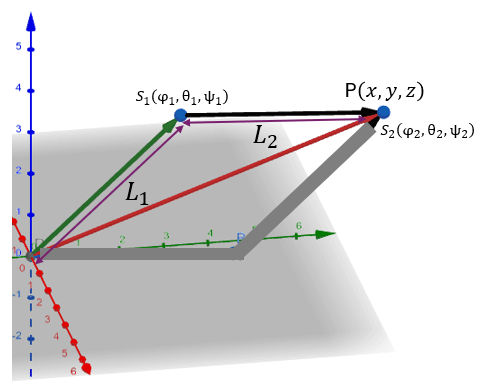
\includegraphics[scale=0.5]{resultante.png}
	\caption{Cálculo de la resultante para obtener la posición del efector final}
	\label{fig:resultante}
\end{figure}